\documentclass[usenames,dvipsnames,tikz]{standalone}
\usepackage{xcolor}
\colorlet{tBlue}{RoyalBlue!35!Cerulean}
\colorlet{tRed}{Red}
\definecolor{tGreen}{HTML}{569909}
\usepackage{tikz}
\usepackage{standalone}
\begin{document}
	
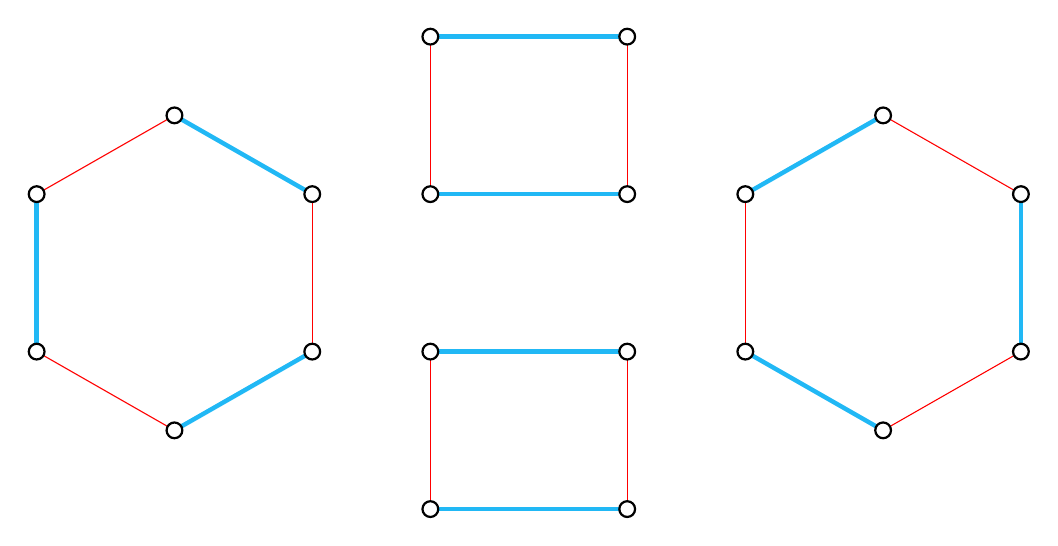
\begin{tikzpicture}
%\draw [help lines] (-1,-1) grid (15, 8);

%C1 - blue
\draw [ultra thick, tBlue] (0.5,3) -- (0.5,5);
\draw [ultra thick, tBlue] (2.25,2) -- (4,3); 
\draw [ultra thick, tBlue] (4,5) -- (2.25,6); 

%C2 - blue
\draw [ultra thick, tBlue] (5.5,5) -- (8,5); 
\draw [ultra thick, tBlue] (5.5,7) -- (8,7);

%C3 - blue
\draw [ultra thick, tBlue] (5.5,1) -- (8,1);
\draw [ultra thick, tBlue] (5.5,3) -- (8,3);

%C4 - blue
\draw [ultra thick, tBlue] (13,3) -- (13,5);
\draw [ultra thick, tBlue] (11.25,2) -- (9.5,3);
\draw [ultra thick, tBlue] (11.25,6) -- (9.5,5);

%-------------------------------

%C1 - red
\draw [tRed] (0.5,3) -- (2.25,2); 
\draw [tRed] (4,3) -- (4,5); 
\draw [tRed] (0.5,5) -- (2.25,6);

%C2 - red
\draw [tRed] (5.5,5) -- (5.5,7);
\draw [tRed] (8,5) -- (8,7);

%C3 - red
\draw [tRed] (5.5,1) -- (5.5,3);
\draw [tRed] (8,1) -- (8,3); 

%C4 - red
\draw [tRed] (13,3) -- (11.25,2);
\draw [tRed] (13,5) -- (11.25,6); 
\draw [tRed] (9.5,3) -- (9.5,5);

%----------------------------

%C1 - vertices
\draw [fill=white, thick] (2.25,2) circle [radius = 0.1]; %v14
\draw [fill=white, thick] (0.5,3) circle [radius = 0.1]; %v7
\draw [fill=white, thick] (4,3) circle [radius = 0.1]; %v18
\draw [fill=white, thick] (0.5,5) circle [radius = 0.1]; %v6
\draw [fill=white, thick] (4,5) circle [radius = 0.1]; %v3
\draw [fill=white, thick] (2.25,6) circle [radius = 0.1]; %v15

%C2 - vertices
\draw [fill=white, thick] (5.5,5) circle [radius = 0.1]; %v4
\draw [fill=white, thick] (8,5) circle [radius = 0.1]; %v8
\draw [fill=white, thick] (5.5,7) circle [radius = 0.1]; %v17
\draw [fill=white, thick] (8,7) circle [radius = 0.1]; %v12

%C3 - vertices
\draw [fill=white, thick] (5.5,1) circle [radius = 0.1]; %v5
\draw [fill=white, thick] (8,1) circle [radius = 0.1]; %v9
\draw [fill=white, thick] (5.5,3) circle [radius = 0.1]; %v16
\draw [fill=white, thick] (8,3) circle [radius = 0.1]; %v12

%C4 - vertices
\draw [fill=white, thick] (11.25,2) circle [radius = 0.1]; %v2
\draw [fill=white, thick] (9.5,3) circle [radius = 0.1]; %v11
\draw [fill=white, thick] (13,3) circle [radius = 0.1]; %v19
\draw [fill=white, thick] (9.5,5) circle [radius = 0.1]; %v10
\draw [fill=white, thick] (13,5) circle [radius = 0.1]; %v20
\draw [fill=white, thick] (11.25,6) circle [radius = 0.1]; %v1

%C1 - labels
%\node [below] at (2,1.5) {$v_{14}$};
%\node [left] at (0,2.6) {$v_7$};
%\node [right] at (4,2.6) {$v_{18}$};
%\node [left] at (0,5) {$v_6$};
%\node [right] at (4,5) {$v_3$};
%\node [above] at (2,6.1) {$v_{15}$};

%C2 - labels
%\node [below] at (5.5,5) {$v_4$};
%\node [below] at (8,5) {$v_8$};
%\node [above] at (5.5,7) {$v_{17}$};
%\node [above] at (8,7) {$v_{13}$};

%C3 - labels
%\node [below] at (5.5,0.6) {$v_5$};
%\node [below] at (8,0.6) {$v_9$};
%\node [above] at (5.5,2.6) {$v_{16}$};
%\node [above] at (8,2.6) {$v_{12}$};


%C4 - labels
%\node [below] at (11.5,1.5) {$v_2$};
%\node [left] at (9.5,2.6) {$v_{11}$};
%\node [right] at (13.5,2.6) {$v_{19}$};
%\node [left] at (9.5,5) {$v_{10}$};
%\node [right] at (13.5,5) {$v_{20}$};
%\node [above] at (11.5,6.1) {$v_1$};

%Component labels
%\node at (2,3.75) {\Large{$C_1$}};
%\node at (6.75,6) {\Large{$C_2$}};
%\node at (6.75,1.6) {\Large{$C_3$}};
%\node at (11.5,3.75) {\Large{$C_4$}};


\end{tikzpicture}
	
\end{document}
